\documentclass{article}
	\usepackage{geometry}
	\usepackage{graphicx}
	\usepackage{indentfirst}
	\usepackage[hyphens]{url}
	\usepackage{listings}
	\usepackage{color}
	\definecolor{gray}{rgb}{0.3,0.3,0.3}
	\usepackage{caption}
	\DeclareCaptionFont{white}{\color{white}}
	\DeclareCaptionFormat{listing}{\colorbox{gray}{\parbox{\textwidth}{#1#2#3}}}
	\captionsetup[lstlisting]{format=listing,labelfont={bf,sf,white},textfont={bf,sf,white}}
	\usepackage{xcolor}
	\usepackage{booktabs}
	\captionsetup[table]{labelfont=bf}
	\usepackage[colorlinks,linkcolor=red]{hyperref}

	\begin{document}
		\begin{center}\textbf{Bo Zhang\\01063214\\}
		\end{center}
		\section{Friendship Paradox with Facebook Account}
		Determine if the friendship paradox holds for my Facebook account. Compute the mean, standard deviation, and median of the number of friends that my friends have. Create a graph of the number of friends (y-axis) and the friends themselves, sorted by number of friends (x-axis). Do include me in the graph and label me accordingly.\\

		\noindent\textbf{Algorithm: }\\
		\indent1. Use the package ``pygraphml''(\url{http://hadim.fr/pygraphml/index.html}) to parse the GraphML file.\\
		\indent2. Read the nodes 1 by 1.\\
		\indent3. For every node, if it has friend\_count, save the friend index and its friend\_count into the csv file.\\
		\indent4. Save my friend\_count into \href{https://github.com/zhangboroy/cs532-s17/blob/master/assg04_submission/facebookFriends.csv}{``facebookFriends.csv''}.\\
		\indent5. Open the csv file in R and read all the data to a table.\\
		\indent6. Delete the row of me and save it to a friends table.\\
		\indent7. Compute the mean, standard deviation, and median of the number of friends with the friends table.\\
		\indent8. Plot the scatter with the full data table.\\

		\noindent\textbf{Source code:}
		\lstinputlisting[language=Python, breakatwhitespace=false), label=graphRead.py, caption=The content of graphRead.py]{graphRead.py}
		\pagebreak

		\lstinputlisting[language=R, breakatwhitespace=false), label=Q1.R, caption=The content of Q1.R]{Q1.R}

		\noindent\\\textbf{Results:}
		\begin{table}[!htb]
			\centering
			\caption{\textbf{My Friend\# v.s. Friends Friend\#}}
			\begin{tabular}{cccc}
				\toprule
				\textbf{Mean} & \textbf{Standard Deviation} & \textbf{Median} & \textbf{Me}\\
				358.987 & 371.5853 & 266.5 & 154\\
				\bottomrule
			\end{tabular}
		\end{table}
		\begin{figure}[!htb]
			\centering 
			\href{https://github.com/zhangboroy/cs532-s17/blob/master/assg04_submission/FacebookFriends.png}
			{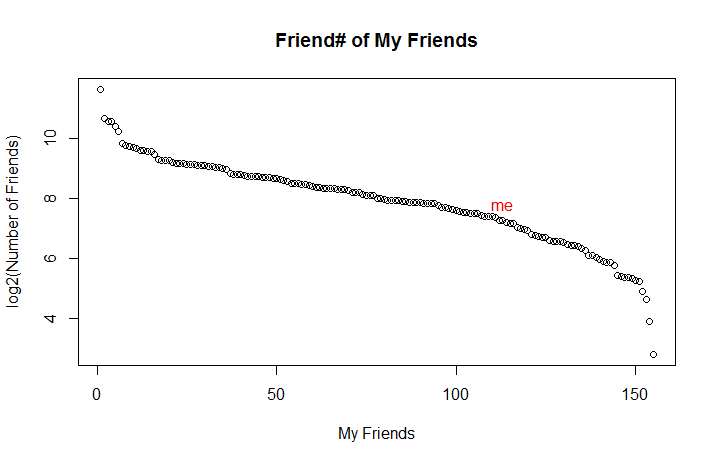
\includegraphics[width=0.9\textwidth]{FacebookFriends.png}}
			\label{fig:Facebook Friends} 
		\end{figure}

		According to these figures, more than 2/3 of ``my'' friends have more friends than ``me'' and the mean is more than double of ``me''. Therefore, the friendship paradox seems hold for ``my'' Facebook account.\\
		\section{Friendship Paradox with Twitter Followers}

		\indent Determine if the friendship paradox holds for your Twitter account. Since Twitter is a directed graph, use ``followers'' as value you measure.\\
		\indent Generate the same graph as in question \#1, and calcuate the same mean, standard deviation, and median values.\\\\
		\textbf{Algorithm:}\\
		\indent1. Use the script from \url{http://stackoverflow.com/questions/31000178/how-to-get-large-list-of-
followers-tweepy} to download the followers\_count of all followers, and save them to \href{https://github.com/zhangboroy/cs532-s17/blob/master/assg04_submission/twitterFollowers.csv}{``twitterFollowers.csv''}.\\
		\indent2. Open the csv file in R and read all the data to a table.\\
		\indent3. Delete the row of me and save it to a friends table.\\
		\indent4. Compute the mean, standard deviation, and median of the number of friends with the friends table.\\
		\indent5. Plot the scatter with the full data table.\\
		\indent6. Use the package ``pygraphml''(\url{http://hadim.fr/pygraphml/index.html}) to parse the GraphML file.\\
		\indent7. Read the lines of the csv file 1 by 1.\\
		\indent8. Split the line into 2 parts and add the first part to the node's id and Label. Add the second part to the node's friend\_count.\\
		\indent9. Save the nodes into \href{https://github.com/zhangboroy/cs532-s17/blob/master/assg04_submission/twitterFollowers.graphml}{``twitterFollowers.graphml''}.\\\\
		\textbf{Source code:}
		\lstinputlisting[language=Python, breakatwhitespace=false), label=downloadTwitterFollowers.py, caption=The content of downloadTwitterFollowers.py]{downloadTwitterFollowers.py}
		\lstinputlisting[language=Python, breakatwhitespace=false), label=graphWrite.py, caption=The content of graphWrite.py]{graphWrite.py}
		\lstinputlisting[language=R, breakatwhitespace=false), label=Q2.R, caption=The content of Q2.R]{Q2.R}

		\noindent\\\textbf{Results: }twitterFollowers.graphml
		\begin{table}[!htb]
			\centering
			\caption{\textbf{My Follower\# v.s. Followers Follower\#}}
			\begin{tabular}{cccc}
				\toprule
				\textbf{Mean} & \textbf{Standard Deviation} & \textbf{Median} & \textbf{Me}\\
				1516.9 & 10183.27 & 311 & 621\\
				\bottomrule
			\end{tabular}
		\end{table}
		\begin{figure}[!htb]
			\centering
			\href{https://github.com/zhangboroy/cs532-s17/blob/master/assg04_submission/TwitterFollowers.png}
			{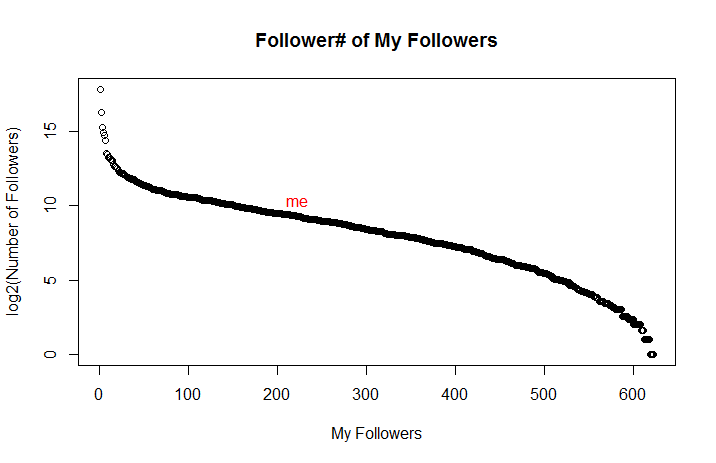
\includegraphics[width=0.9\textwidth]{TwitterFollowers.png}}
			\label{fig:Twitter Followers} 
		\end{figure}

		According to these figures, about 2/3 of ``my'' followers have less followers than ``me'' although the mean is more than double of ``me''. Therefore, the friendship paradox seems not hold for ``my'' twitter account measured by ``followers''.\\
		\section{Friendship Paradox with LinkedIn Connections}
		Repeat question \#1, but with your LinkedIn profile.\\\\
		\textbf{Method \& Algorithm:}\\
		\indent1. Use Octoparse(a Web Scraping Tool) to get all my connections' profile page links. Open the page of ``My Connections''(When using this tool, must click the link from another page. If opening this page directly from the address bar, the connections will be incomplete.), then extract the texts with my connections' profile page links and save it to \href{https://github.com/zhangboroy/cs532-s17/blob/master/assg04_submission/linkedinConnections.txt}{``linkedinConnections.txt''}.\\
		\indent2. Open the TXT file with python, extract the link part, complete it with domain and save it to \href{https://github.com/zhangboroy/cs532-s17/blob/master/assg04_submission/linkedinContactLinks.txt}{``linkedinContactLinks.txt''}.\\
		\indent3. Use Octoparse to open all these links, extract the connections number and save it to \href{https://github.com/zhangboroy/cs532-s17/blob/master/assg04_submission/linkedinConnectionsNumber.txt}{``linkedinConnectionsNumber.txt''}.\\
		\indent4. Open the TXT file with python, manipulate the data and save it to \href{https://github.com/zhangboroy/cs532-s17/blob/master/assg04_submission/linkedinConnections.csv}{``linkedinConnections.csv''}(Because the connection number actually count self in and when the connection number is larger than 500, it shows 500+).\\
		\indent5. Open the csv file in R and read all the data to a table.\\
		\indent6. Delete the row of me and save it to a friends table.\\
		\indent7. Compute the mean, standard deviation, and median of the number of friends with the friends table.\\
		\indent8. Plot the scatter with the full data table.\\\\
		\textbf{Source code:}
		\lstinputlisting[language=Python, breakatwhitespace=false), label=extractLinkedinContactLinks.py, caption=The content of extractLinkedinContactLinks.py]{extractLinkedinContactLinks.py}
		\lstinputlisting[language=Python, breakatwhitespace=false), label=linkedinConnectionsEdit.py, caption=The content of linkedinConnectionsEdit.py]{linkedinConnectionsEdit.py}
		\lstinputlisting[language=R, breakatwhitespace=false), label=Q3.R, caption=The content of Q3.R]{Q3.R}

		\noindent\\\textbf{Results:}
		\begin{table}[!htb]
			\centering
			\caption{\textbf{My Connection\# v.s. Connections Connection\#}}
			\begin{tabular}{cccc}
				\toprule
				\textbf{Mean} & \textbf{Standard Deviation} & \textbf{Median} & \textbf{Me}\\
				339.0294 & 181.3933 & 481 & 68\\
				\bottomrule
			\end{tabular}
		\end{table}
		\begin{figure}[!htb]
			\centering 
			\href{https://github.com/zhangboroy/cs532-s17/blob/master/assg04_submission/linkedinConnections.png}
			{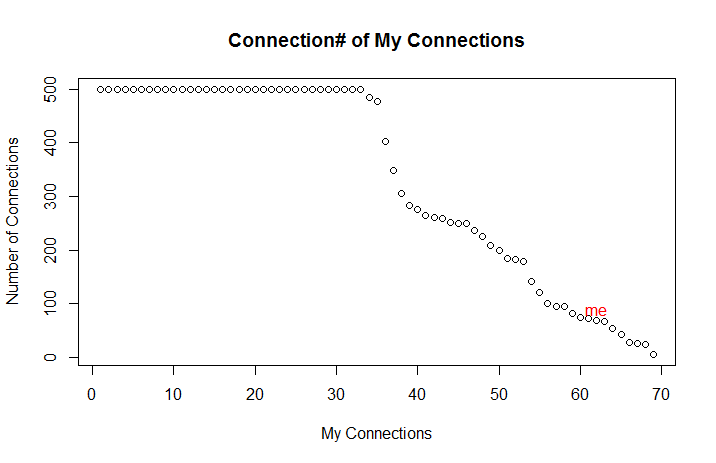
\includegraphics[width=0.9\textwidth]{linkedinConnections.png}}
			\label{fig:LinkedinConnections} 
		\end{figure}

		According to these figures, nearly 90\% of my connections have more connections than me and the mean is nearly 5 times of me. Therefore, the friendship paradox seems hold for my LinkedIn profile.\\
		\section{Friendship Paradox with Facebook Profile}
		Repeat question \#1, but with your own facebook profile. Explain in detail how you got the information.\\\\
		\textbf{Answer: }I don't have a facebook account.\\
		\section{Friendship Paradox with Twitter Following}Repeat question \#2, but change ``followers'' to ``following''.\\\\
		\textbf{Algorithm:}\\
		\indent1. Use the script from \url{http://stackoverflow.com/questions/31000178/how-to-get-large-list-of-
followers-tweepy}, but replace the followers\_count of all followers with friends\_count of all friends, and save them to \href{https://github.com/zhangboroy/cs532-s17/blob/master/assg04_submission/twitterFollowing.csv}{``twitterFollowing.csv''}.\\
		\indent2. Open the csv file in R and read all the data to a table.\\
		\indent3. Delete the row of me and save it to a friends table.\\
		\indent4. Compute the mean, standard deviation, and median of the number of friends with the friends table.\\
		\indent5. Plot the scatter with the full data table.\\
		\indent6. Use the package ``pygraphml''(\url{http://hadim.fr/pygraphml/index.html}) to parse the GraphML file.\\
		\indent7. Read the lines of the csv file 1 by 1.\\
		\indent8. Split the line into 2 parts and add the first part to the node's id and Label. Add the second part to the node's friend\_count.\\
		\indent9. Save the nodes into the \href{https://github.com/zhangboroy/cs532-s17/blob/master/assg04_submission/twitterFollowing.graphml}{``twitterFollowing.graphml''}.\\\\
		\textbf{Source code:}
		\lstinputlisting[language=Python, breakatwhitespace=false), label=downloadTwitterFollowering.py, caption=The content of downloadTwitterFollowering.py]{downloadTwitterFollowering.py}
		\lstinputlisting[language=Python, breakatwhitespace=false), label=graphWrite.py, caption=The content of graphWrite.py]{graphWrite.py}
		\lstinputlisting[language=R, breakatwhitespace=false), label=Q5.R, caption=The content of Q5.R]{Q5.R}

		\noindent\\\textbf{Results: }twitterFollowing.graphml
		\begin{table}[!htb]
			\centering
			\caption{\textbf{My Following\# v.s. Followings Following\#}}
			\begin{tabular}{cccc}
				\toprule
				\textbf{Mean} & \textbf{Standard Deviation} & \textbf{Median} & \textbf{Me}\\
				859.4967 & 4892.806 & 256 & 304\\
				\bottomrule
			\end{tabular}
		\end{table}
		\begin{figure}[!htb]
			\centering 
			\href{https://github.com/zhangboroy/cs532-s17/blob/master/assg04_submission/TwitterFollowings.png}
			{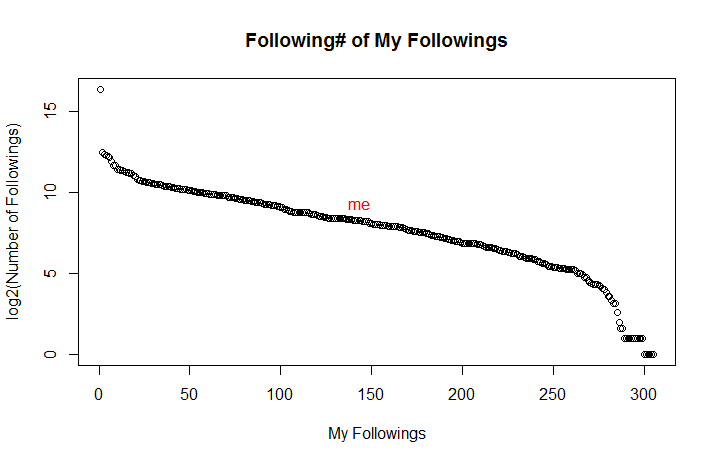
\includegraphics[width=0.9\textwidth]{TwitterFollowings.png}}
			\label{fig:Twitter Followings} 
		\end{figure}

		According to these figures, more than half of ``my'' followings have less followings than ``me'' although the mean is nearly triple of ``me''. Therefore, the friendship paradox seems not hold for ``my'' twitter account measured by ``followering''.\\
	\end{document}